\chapter{1982:Robert Endre Tarjan}
\label{chap:tarjan}
\begin{center}
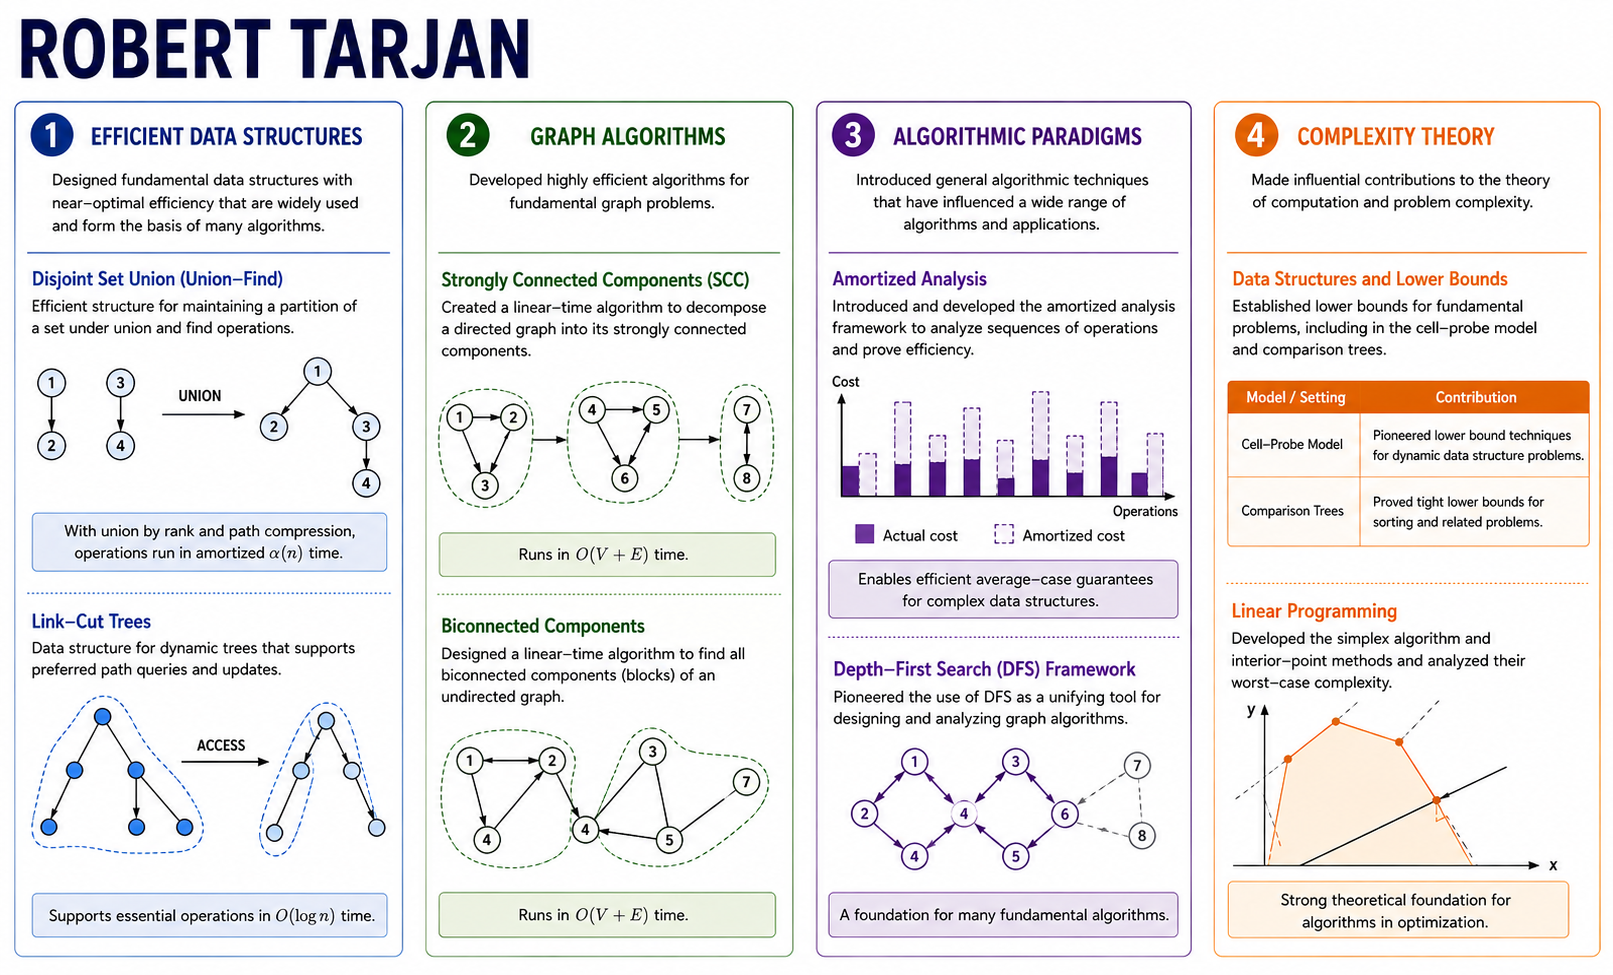
\includegraphics[width=\textwidth]{infographics/abacus1.png}
\end{center}
\expandedchapterspacing
\index{Tarjan, Robert Endre}
\booknote{The central habit in this chapter is to let a data structure remember the past, and to judge an algorithm over a whole \emph{sequence} of operations rather than one isolated step.}

\section{An Opening Story: Joining Clubs and Checking Roads}
Six friends---Alice, Bob, Carol, Dave, Eve, and Frank---start in six separate clubs, each with one member. They begin merging: Alice and Bob form one club, Carol and Dave form another, then Bob and Carol merge their two clubs. Now the question is asked: ``Are Alice and Dave in the same club?''

If the computer stores each club as a list of members, answering takes two list scans and an easy check. But suppose the clubs keep merging until thousands of people are involved. Every merge can force a list to be walked end to end, and every query may scan a large list. A program built this way can become unusable long before the problem itself is complicated. The simple question---who belongs to whom---hides a design decision: \emph{what information should the program remember between questions?}

The same issue appears for roads. A map of towns and roads is a \emph{graph}: points (\emph{vertices}) joined by lines (\emph{edges}). A \emph{bridge} is a road whose removal would split the map into two disconnected halves. How can we find every bridge without testing each road by hand?

Tarjan's 1982 Rolf Nevanlinna Prize recognized two answers that now appear in nearly every computer science curriculum: the \emph{union--find} data structure with amortized analysis, and \emph{depth-first search} with its discovery and low-link numbers. Both answers share one philosophy: the structure should record a small, provably correct summary of the past, and the running time should be measured over a whole sequence of operations.

\section{The Problem}
Two problems, both phrased as questions a computer must answer fast.

\noindent\textbf{Union--find.} We maintain a collection of disjoint sets of items. Two operations are allowed:
\begin{itemize}
\item \textsc{find}(x): return the name of the set containing $x$;
\item \textsc{union}(x,y): merge the sets containing $x$ and $y$.
\end{itemize}
A sequence of $m$ operations on $n$ items arrives, one after another. How much total time is needed? The naive list approach is easy but can be catastrophically slow on long sequences.

\noindent\textbf{Graph exploration.} Given a graph, find all bridges, articulation points (vertices whose removal disconnects the graph), and, for directed graphs, strongly connected components (maximal groups in which every vertex can reach every other). A correct but naive method---remove each edge and re-search---repeats a global computation $m$ times.

The problems look unrelated: one is about organizing data, the other about exploring a graph. The connection is that both were stuck because nobody had the right way to \emph{measure} cost and the right thing to \emph{remember}.

\section{The World Before}
In the early decades of computer science, memory was expensive, processors were slow, and an algorithm was typically judged by its worst-case performance on a single operation. Two consequences followed.

\noindent\textbf{Union--find as linked lists.} The natural implementation stores each set as a linked list. A \textsc{find} walks the list of the item's set; a \textsc{union} walks one list to its tail and attaches the other list. This is easy to describe and correct. But consider merging $n$ singletons into one set by always appending the whole current set to the next item: the growing list is walked once per merge, costing about $n^2/2$ steps. Each \textsc{union} is individually cheap---except when it is the $n$-th one---and every earlier merge looks fine in isolation. There was no language for saying: ``this particular operation is expensive, but that is fine because it can only happen rarely.''

\noindent\textbf{Finding bridges by deletion.} To test whether a road is a bridge, remove it and check whether the two endpoints are still connected. Repeating this for every edge of a graph with $m$ edges costs about $m$ full connectivity searches. On a large road map, that is hopeless. The naive algorithm works on paper but reveals nothing about the structure that makes some roads fragile and others not.

The missing ingredients were two ideas that seem obvious in hindsight:
\begin{enumerate}
\item \emph{Amortized analysis}: judge a sequence of operations, and let rare expensive operations be paid for by many cheap ones.
\item \emph{Reusable certificates}: a graph exploration should record exactly the information a later decision needs, not re-derive it from scratch.
\end{enumerate}

\section{The New Idea}
\subsection{Union--find: sets as shallow trees}
Store each set as a rooted tree, with every item pointing to its parent and a root pointing to itself. \textsc{find}(x) climbs from $x$ to its root and returns it. \textsc{union}(x,y) finds both roots and attaches one under the other.

Two refinements make the trees stay shallow:
\begin{itemize}
\item \textbf{Union by rank.} Each root carries a \emph{rank}, roughly the height of its tree. Always attach the smaller-rank root under the larger-rank one. This alone guarantees that every tree has height at most $\log_2 n$, so a single \textsc{find} never costs more than $O(\log n)$.
\item \textbf{Path compression.} During \textsc{find}(x), every vertex on the path from $x$ to the root is re-pointed directly at the root. The mathematical partition is unchanged---the representative is the same---but future queries along that path become one step each. The query \emph{rewrites the structure to make later work cheaper}.
\end{itemize}

The second refinement is the surprising one. A query that ``only asks a question'' actively improves the data structure. That is only safe if the improvement preserves the invariant that makes answers correct. It does: pointing a vertex at its root does not change which set any item belongs to.

\subsection{Amortized analysis: the bank account}
To understand why the combination is fast, forget single operations. Think of a bank account. Cheap operations deposit credit; an expensive operation spends the accumulated credit. An analysis is successful if we can prove the balance never goes negative.

Formally, assign a number $\Phi$ (the \emph{potential}) to the current state of the data structure. If operation $i$ costs $c_i$ and changes the potential from $\Phi_{i-1}$ to $\Phi_i$, its \emph{amortized} cost is defined as
\[
\widehat c_i=c_i+\Phi_i-\Phi_{i-1}.
\]
Summing over a whole sequence makes the potential terms telescope, so the total real cost equals the total amortized cost plus a boundary term. If the potential is nonnegative and each $\widehat c_i$ is small, the whole sequence is cheap. This is the mathematical version of the bank account: an expensive operation is charged for \emph{raising} the potential, and later cheap operations are the ones that spend it.

For union--find, the potential measures how ``squashed'' the trees are. Path compression is expensive when it flattens a long path, but it buys a large improvement in the forest; union by rank ensures that any one vertex cannot be moved into a better position too many times.

\subsection{Depth-first search: two numbers as a certificate}
Start at any vertex and follow one unexplored road at a time, turning back only when you reach a dead end. Number each vertex (\emph{disc}, for discovery time) in the order it is first reached. While searching, also record, for each vertex $v$, the number
\[
\operatorname{low}(v)=\text{the smallest discovery time reachable from the subtree under }v
\]
using tree edges followed by at most one non-tree edge. In words: \emph{how far back can this part of the map return, without retracing the parent road?} This is the undirected low-link quantity; for directed strongly connected components, Tarjan's algorithm uses a related low-link value that tracks edges to vertices still on the active search stack.

Two inequalities now read like the whole answer:
\begin{itemize}
\item if a child $w$ of $v$ has $\operatorname{low}(w)>\operatorname{disc}(v)$, then the road $v$--$w$ is a bridge (the subtree under $w$ cannot return to $v$ or above);
\item if $\operatorname{low}(w)\geq\operatorname{disc}(v)$, then removing $v$ separates that child's subtree from the rest (the subtree can return to $v$ itself, but not above it).
\end{itemize}
One pass over the graph produces all bridges and articulation points; with the directed-graph low-link variant and a stack, the same depth-first-search framework also produces strongly connected components. The discovery numbers and low-links are the certificate: they summarize an enormous family of possible return paths without listing them.

\section{How It Works: Worked Examples}
\subsection{A warm-up: amortization with a growing array}
Before union--find, see amortization on a friendlier object. A dynamic array must grow when it is full. Doubling the size and copying every item costs $O(n)$ when the array holds $n$ items, which sounds expensive. But over $m$ appends, the array doubles only about $\log_2 m$ times, and the total copying is
\[
1+2+4+\cdots+2^{\lceil\log_2 m\rceil}=O(m).
\]
The expensive rebuilds are paid for by the many cheap appends that filled the old block. Each append has amortized cost $O(1)$. This is the same accounting that makes path compression work.

\subsection{Union--find on six people, step by step}
Start with $A,B,C,D,E,F$, each in its own set.

\begin{enumerate}
\item \textsc{union}(A,B): both roots have rank $0$; attach $A$ below $B$. Tree: $A\to B$.
\item \textsc{union}(C,D): similarly, $C\to D$.
\item \textsc{union}(B,D): roots $B$ and $D$ have equal rank; attach $B$ below $D$. Now $A\to B\to D$ and $C\to D$. Root: $D$.
\item \textsc{find}(A): climb $A\to B\to D$ and return $D$. Path compression re-points $A$ and $B$ directly at $D$. The next \textsc{find}(A) or \textsc{find}(B) costs one step.
\item \textsc{union}(E,F): $E\to F$.
\item \textsc{find}(A) vs.\ \textsc{find}(E): returns $D$ and $F$---different clubs.
\end{enumerate}

Without path compression, step 4 would leave the chain $A\to B\to D$ intact forever. With it, the query paid for a permanent shortcut. If a club merge later asks for \textsc{find}(A) a hundred times, the first costs three steps and the remaining ninety-nine cost one each.

\subsection{A bridge hunt with depth-first search}
Take the graph with edges
\[
(a,b),(b,c),(c,a),(c,d),(d,e),(e,f),(f,d).
\]
Explore from $a$, always taking the alphabetically first unexplored road.

\begin{center}
\begin{tabular}{lcc}
\toprule
Vertex & \textsc{disc} & \textsc{low} \\
\midrule
$a$ & 1 & 1 \\
$b$ & 2 & 1 \\
$c$ & 3 & 1 \\
$d$ & 4 & 4 \\
$e$ & 5 & 4 \\
$f$ & 6 & 4 \\
\bottomrule
\end{tabular}
\end{center}

How the low-links are computed, from the leaves upward. Vertex $f$ has a back edge to $d$ (discovery time 4), so $\operatorname{low}(f)=4$. Vertex $e$ sees its child $f$ reaching 4, so $\operatorname{low}(e)=4$. Vertex $d$'s subtree reaches 4 and no further, so $\operatorname{low}(d)=4$. Vertex $c$ has a back edge to $a$ (time 1), so $\operatorname{low}(c)=1$, and this value propagates up through $b$.

Now test the bridges:
\begin{itemize}
\item edge $c$--$d$: is $\operatorname{low}(d)=4>\operatorname{disc}(c)=3$? Yes. The subtree $\{d,e,f\}$ cannot return above $c$---bridge. This matches intuition: the triangle on $a,b,c$ and the cycle on $d,e,f$ are joined only by $c$--$d$.
\item edge $e$--$f$: $\operatorname{low}(f)=4>\operatorname{disc}(e)=5$? No. Within a cycle, no single road is a bridge.
\end{itemize}
The search never tests every alternative route. It asks, once per tree edge, whether the child's subtree can climb back over the parent road. The two numbers $\operatorname{disc}$ and $\operatorname{low}$ contain exactly the information needed and no more.

\section{The Mathematics in Brief}
The famous union--find guarantee is
\[
O(m\,\alpha(n))
\]
for $m$ operations on $n$ items, where $\alpha$ is the \emph{inverse Ackermann function}. This function grows so slowly that it is at most $4$ for any number of atoms in the universe. The notation is a compact record of a real theorem: the total pointer changes across all unions and finds are almost linear. The proof groups vertices by rank and shows that a vertex can be redirected only through a tiny hierarchy of rapidly expanding rank classes. The intuition is simple even when the hierarchy is not: \emph{every expensive flattening buys a large, durable improvement in the vertex's future position.}

For depth-first search, the inequalities
\[
\operatorname{low}(w)>\operatorname{disc}(v)\quad\Longrightarrow\quad \text{edge }v\text{--}w\text{ is a bridge}
\]
and
\[
\operatorname{low}(w)\geq\operatorname{disc}(v)\quad\Longrightarrow\quad v\text{ is an articulation point for that branch}
\]
turn a visual idea about fragile networks into a checkable algorithm. The strict versus non-strict inequality is exactly the difference between ``the subtree can return to $v$ but not above it'' and ``it cannot even reach $v$ again.''

Depth-first search also produces certificates for directed graphs. A stack holds vertices of the search branch currently being explored. When a vertex is identified as the root of a strongly connected component (its low-link equals its discovery time), popping until the root removes exactly one complete component. Each vertex and edge is pushed, inspected, and removed a bounded number of times, so the whole algorithm runs in linear time.

\section{Limits and Modern Views}
The classical guarantees depend on implementation details. A careless union rule creates tall trees and destroys the near-linear bound. If parallel edges are stored without identifiers, a bridge test can mistake one copy of a doubled road for the parent edge. Recursive depth-first search can exhaust the call stack on a very long path; an iterative version must store its own exploration state. The lesson is that the invariant must be stated before the code is written.

Two modern settings push beyond the classical picture:
\begin{itemize}
\item \textbf{Dynamic graphs.} Real networks change: a road closes, a dependency is deleted. Re-running a linear algorithm after every update is too slow. Deletions are the hard case because an edge that once supported connectivity can vanish. The low-link invariant does not survive a deletion automatically, so dynamic connectivity maintains richer structures---spanning forests, balanced trees, randomized sampling---while asking the same Tarjan-style question: \emph{what summary of the past is enough to repair the answer after a local change?}
\item \textbf{Parallelism.} Depth-first search is sequential in its purest form, because the next branch depends on which vertices are already marked. Connectivity and union operations parallelize better, but synchronization and memory traffic become part of the real cost. An asymptotically optimal algorithm can lose to a worse one on real hardware if its operations are hard to distribute.
\end{itemize}

The design philosophy survives all these changes: use a small, explicit certificate of the past to make a large future computation cheap. The certificate may be a parent pointer, a rank, a discovery time, or a low-link value. Its power comes from the proof that it is exactly the information later decisions require \cite{tarjan-union,tarjan-dfs}.

\section{Exercises and Self-Study Guide}
\begin{enumerate}[label=\textbf{E\arabic*.}]
\item Run \textsc{union} by rank and \textsc{find} with path compression on the people $A,B,C,D,E,F$ with merges $(A,C)$, $(E,D)$, $(B,F)$, $(C,D)$, $(F,A)$. Draw the forest after each merge.
\hint{Attach the smaller-rank root under the larger; remember that path compression happens only inside \textup{\textsc{find}}.}
\item Show that merging $n$ singletons into one set by the linked-list method can cost about $n^2/2$ steps.
\hint{Keep merging the growing list into the next singleton, and count how many times the growing list is walked.}
\item Prove, from the low-link definition, that $\operatorname{low}(w)>\operatorname{disc}(v)$ forces the tree edge $v$--$w$ to be a bridge.
\hint{If removing $v$--$w$ still left the graph connected, some path from the subtree under $w$ to the outside would exist; trace how low-link would then reach $\operatorname{disc}(v)$ or less.}
\item On the graph $(a,b),(b,c),(c,a),(c,d)$, run depth-first search from $a$ and compute all discovery and low-link numbers. Where is the articulation point?
\hint{Follow the same table format as the worked example. Check which child $w$ of $c$ satisfies $\operatorname{low}(w)\geq\operatorname{disc}(c)$.}
\item Design a potential function that proves the amortized $O(1)$ append cost of a doubling array.
\hint{Let the potential be the number of occupied slots beyond half the array's capacity.}
\item Kruskal's minimum-spanning-tree algorithm accepts edges from lightest to heaviest, adding an edge exactly when its endpoints lie in different components. Explain which two invariants prove correctness and which data structure provides the speed.
\hint{Separate ``the accepted edges form a forest'' from ``each accepted edge is the lightest across a cut.'' Union--find maintains only the component information the first invariant needs.}
\end{enumerate}

\booknote{A final exercise in judgment: whenever a query operation improves the structure for the future, check which invariant guarantees the improvement is invisible to the answers. If you cannot name that invariant, the optimization is not safe.}
\clearpage
